\documentclass[11pt]{report}
%\usepackage{fancybox}
\usepackage{geometry}
\usepackage{amsmath}
\usepackage{txfonts}
\usepackage{layout}
\usepackage{setspace}
%\usepackage{mathptmx}
\geometry{a4paper, left=22mm, right=22mm, top=25mm, bottom=25mm}
\usepackage{wrapfig}
\usepackage[dvipdfm]{graphicx,hyperref}
\usepackage{mediabb}
\setstretch{1.3}
\title{\Huge\bf{Role of Noncollective Excitations in Low-Energy Heavy-Ion Fusion Reaction
and Quasi-Elastic Scattering}}
\author{\\\\\\\\\\\\\\\\\\\\\\\\\\\\{\it\Large Department of Physics, Faculty of Science, Tohoku University}\\\\
\Huge Shusaku Yusa}
\date{March, 2013}
\begin{document}


\chapter{Nuclear excitations}
In this chapter, a fundamental feature of nuclear excited states is reviewed.
One can classify the nuclear excitations into two classes, that is, collective
excitations and noncollective excitations.
Properties and differences of these two kinds of excitations are presented.

\section{Collective excitations}
Collective excitations are understood as a collective motion of nucleons
composing a nucleus. There are two kinds of collective excitations, that is,
low-lying collective excitations and giant resonances. 
In this section, we review the low-lying collective excitations since they play
an important role in the low-energy heavy-ion reactions. On the other hand,
the giant resonances appear in the energy region
of ten to several tens of MeV as a
broad resonance. The effect of these high-lying excited states can be
compensated by renormalizing the potential, which will be
discussed in the next chapter.

The most remarkable feature of the collective excitations is a large
electromagnetic transition strength, compared to a single-particle excitation.
Let us consider an electric quadrupole transition 
from a state with spin $I+2$ to a
state with spin $I$ (E2 transition).
The transition probability is given by\cite{RS}
\begin{eqnarray}
  T = \frac{4\pi}{75}\frac{1}{\hbar}
      \left(\frac{E_{\gamma}}{\hbar c}\right)^5
      B(E2,I+2\rightarrow I).
\end{eqnarray}
Here, $E_{\gamma} = E_i - E_f$
is the energy difference of the initial and the final states
and $B(E2,I+2\rightarrow I)$ is called the reduced transition probability.
In general, for a transition from a state $|i\rangle$ with spin $I_i$ to a state $|f\rangle$
with spin $I_f$, the reduced transition probability is given by
\begin{eqnarray}
  B(E\lambda,I_i\rightarrow I_f) = \frac{1}{2I_i+1}
            \left|\langle f||Q_{\lambda}||i\rangle \right|^2,
  \label{BE}
\end{eqnarray}
where, $Q_{\lambda}$ is an electric multipole operator
with a multipolarity $\lambda$ (the E2 transition corresponds to
$\lambda = 2$).
In order to evaluate the magnitude of $B(E\lambda)$-values, 
the Weisscopf unit is often used\cite{BM1} which is give by
\begin{eqnarray}
B_{\rm W}(E\lambda) = \frac{e^2}{4\pi}\left(\frac{3}{\lambda+3}\right)^2
R^{2\lambda},
\end{eqnarray}
where $R = 1.2 A^{1/3}$ (fm) is the radius of the nucleus.
This formula is obtained by assuming
a transition of a nucleon between single-particle levels
and a constant nucleon wave function extending inside the
radius of $R$.
Thus the comparison with this value 
provides an idea on how collective the state is.
If one considers a transition from a $2^+$
state to a $0^+$ state, then the reduced
transition probability is given by
\begin{eqnarray}
  B_{\rm W}(E2) = \frac{e^2}{4\pi}\left(\frac{3}{5}\right)^2R^{4}
        = 30A^{4/3}e^2 {\rm fm}^4
  \label{sptrans}.
\end{eqnarray}
Experimentally obtained B(E2) values
from the first $2^+$ state to the ground state 
are plotted in Fig.\ref{figE2} for various even-even 
nuclei in the Weisscopf unit\cite{BM2}.
One can notice that all the values are greater than one, and quite large for
nuclei in the region of $140\lesssim A\lesssim 180$ and $A \gtrsim 230$.
Nuclei in these region are known to be deformed, and thus the first 
$2^+$ state is a rotational state. 
Reflecting the collective character of these
states, the transition probabilities have a large value.
\begin{figure}[t]
  \begin{center}
    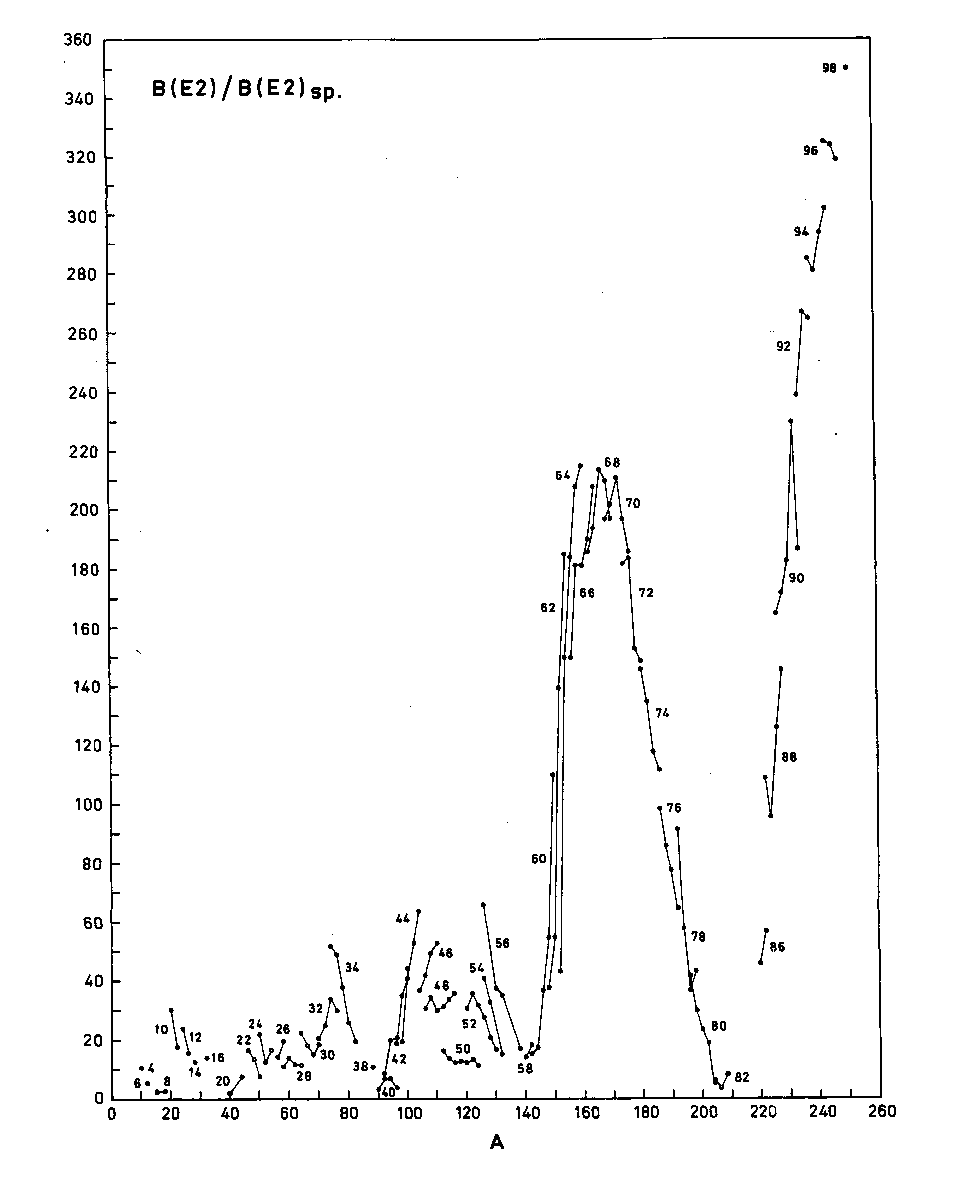
\includegraphics[clip, keepaspectratio,width=120mm]{figure/chapter2/BE2.eps}
    \caption{$B(E2)$ value for various even-even nuclei.
    The $B(E2)$ values are measured in the
    Weisscopf unit. Taken from Ref. \cite{BM2}.}
    \label{figE2}
  \end{center}
\end{figure}

A characteristic feature of the collective states is also found from their
appearance in nuclear spectrum.
Typical nuclear spectra for vibrational and rotational levels are shown
in Figs. \ref{vib_spectrum} and \ref{rot_spectrum}, respectively.
In Fig.\ref{vib_spectrum}, the first $2^{+}$ state and the triplet
states of ${0^+,2^+,4^+}$ appear in $^{106}$Pd and $^{114}$Cd 
in nearly equi-distance. In
Fig.\ref{rot_spectrum}, states with even spin ($I=0,2,4,\cdots$) regularly appear according
to the $E_I \propto I(I+1)$ law.
\begin{figure}[t]
  \begin{center}
    \begin{minipage}[t]{85mm}
      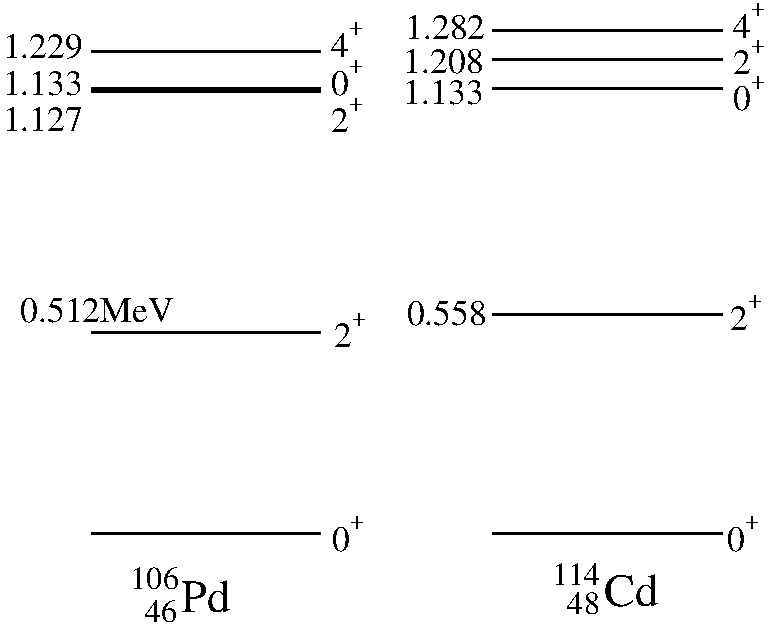
\includegraphics[clip,keepaspectratio,width=85mm]{figure/chapter2/vib_levels.pdf}
      \caption{Vibrational levels.}
      \label{vib_spectrum}
    \end{minipage}
    \hspace{0.5cm}
    \begin{minipage}[t]{70mm}
       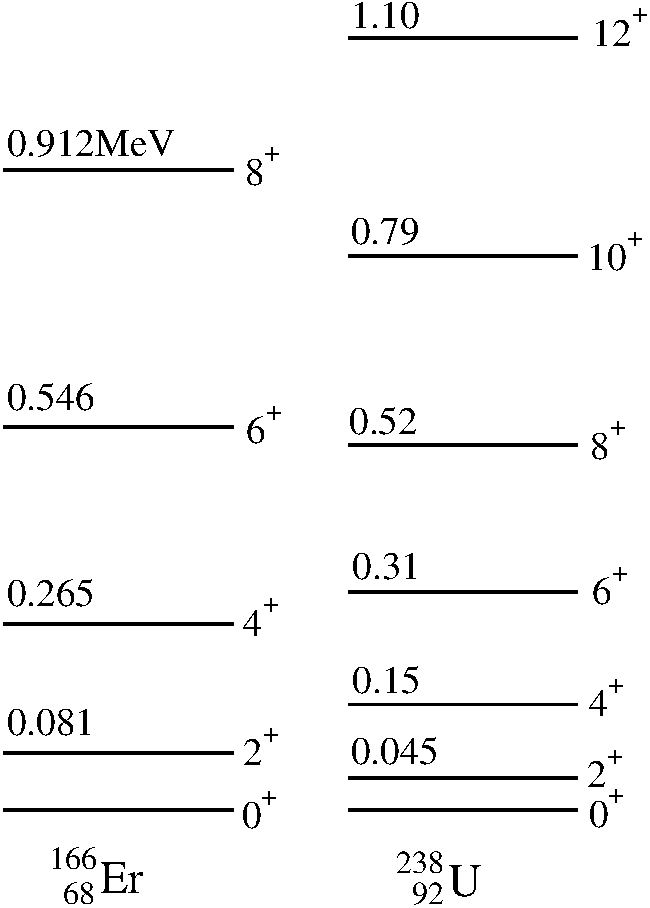
\includegraphics[clip,keepaspectratio,width=70mm]{figure/chapter2/rot_levels.pdf}
       \caption{Rotational levels.}
       \label{rot_spectrum}
    \end{minipage}
  \end{center}
\end{figure}
In the following, we explain how the regularity of these states arises from the
vibrational or rotational properties of the nuclei.

Let us first consider a surface vibration of even-even spherical 
nuclei in a liquid drop model\cite{RS}.
One can expand the distance $R(\theta, \phi)$ from the center-of-mass of
the nucleus to a surface point at angle $(\theta, \phi)$ direction
by spherical harmonics as
\begin{eqnarray}
  R(\theta,\phi) = R_0\left\{1+\sum_{\lambda,\mu}\alpha^{*}_{\lambda \mu }
                   Y_{\lambda \mu }(\theta,\phi)\right\},
   \label{radial}
\end{eqnarray}
where $\alpha_{\lambda\mu}$ is the expansion coefficient.
In the liquid drop model, the surface vibration is described by regarding
the expansion coefficients $\alpha_{\lambda\mu}$ as dynamical variables.
The Hamiltonian for this model is given by
\begin{eqnarray}
  H = \sum_{\lambda,\mu}\left(
      \frac{1}{2}B_\lambda|\dot{\alpha}_{\lambda \mu }|^2
      + \frac{1}{2}C_\lambda|\alpha_{\lambda \mu }|^2
      \right).
   \label{collham}
\end{eqnarray}
Here, the dot means the differentiation with respect to time. The first term
represents the kinetic energy of the vibrational motion and the second term
represents the potential energy associated with the deviation of the nuclear
shape from sphere.
Since this is a Hamiltonian for a harmonic oscillator,
it can be quantized in the
usual manner and reads
\begin{eqnarray}
  H = \sum_{\lambda,\mu}
      \frac{1}{2}\hbar\omega_{\lambda}
      \left(b^{\dagger}_{\lambda \mu }b_{\lambda \mu }+\frac{1}{2}\right),
\end{eqnarray}
where $\omega_\lambda=\sqrt{C_\lambda/B_\lambda}$ and
$b_{\lambda \mu }^{\dagger}$ and ${b}_{\lambda \mu }$ are the
creation and annihilation operators of a phonon with angular momentum 
$\lambda, \mu$.
They satisfy the following commutation relations
\begin{align}
 [b_{\lambda \mu },b_{\lambda^{\prime}\mu^{\prime}}^{\dagger}] 
      &= \delta_{\lambda \lambda^{\prime}}\delta_{\mu\mu^{\prime}}
      \label{commute1},\\
 [b_{\lambda \mu },b_{\lambda^{\prime}\mu^{\prime}}] &= 0
      \label{commute2},\ \ \ \  \\
 [b_{\lambda \mu }^{\dagger},b_{\lambda^{\prime}\mu^{\prime}}^{\dagger}] &= 0.
      \label{commute3}
\end{align}
The first excited state is obtained by creating a phonon in the vacuum
$|0\rangle$
\begin{eqnarray}
  b_{\lambda \mu }^{\dagger}|0\rangle.
\end{eqnarray}
The energy of this state is $\hbar\omega_{\lambda}$ and the spin and the parity are
given by $\lambda$ and $(-1)^{\lambda}$, respectively.
For $\lambda = 2$, the
spin-parity of the first excited state is $2^+$
for even-even nuclei, in which the ground state has $0^+$.
The second excited states are then obtained by creating a phonon on the first
excited state. Again, let us consider the case of $\lambda = 2$. The second
excited state with angular momentum $I,M$ is given by
\begin{eqnarray}
  \frac{1}{\sqrt{2}}\sum _{\mu _1,\mu _2}\langle 2\mu _12\mu _2|IM\rangle
          b_{2\mu _1}^{\dagger}b_{2\mu _2}^{\dagger}|0\rangle.
\end{eqnarray}
From (\ref{commute3}) and a property of Clebsch-Gordan coefficients
\begin{eqnarray}
 \langle 2\mu_1 2\mu_2 | IM\rangle 
       = (-1)^{-I}\langle 2\mu_2 2\mu_1 | IM\rangle,
\end{eqnarray}
one can show that only the states with $I=0,2,4$ are realizable and
all of the three states are degenerated with the energy $2\hbar\omega_2$.
From this consideration, the excited states shown in Fig.\ref{vib_spectrum} are
understood as the quadrupole phonon states, while the triplet of the double
phonon states are split up a little. This split of the spectra 
indicates the deviation from a pure harmonic oscillator.

In the collective model,
one can relate the $B(E\lambda)$ to the
deformation parameter. 
As we will see in Sec. 3.6.1, the electric multipole operator is
calculated as
\begin{eqnarray}
Q_{\lambda\mu} = \frac{3Ze}{4\pi}
R^\lambda\alpha_{\lambda\mu}
\label{Qlam}
\end{eqnarray}
for a sharp-cut density
and $\alpha_{\lambda\mu}$ is related to the deformation parameter
$\beta_{\lambda}$ as
\begin{eqnarray}
\alpha_{\lambda\mu} = \frac{\beta_{\lambda}}{\sqrt{2\lambda+1}}
\left(b_{\lambda\mu}^\dagger + (-1)^\mu b_{\lambda\mu} \right).
\label{alpha_lam}
\end{eqnarray}
The reduced transition probability from $I_i=0$ to $I_f=\lambda$
then becomes
\begin{align}
B(E\lambda, 0\rightarrow\lambda)
&= \left| \langle \lambda || Q_{\lambda} || 0 \rangle \right|^2 \nonumber\\
&= (2\lambda+1) 
\left| \langle \lambda 0 | Q_{\lambda 0} |0 0 \rangle \right|^2
\nonumber\\
&= \left(
\frac{3e}{4\pi}ZR^{\lambda}\beta_{\lambda}
\right)^2.
\label{BE_and_beta}
\end{align}
Thus, one can estimate the deformation parameter from the $B(E\lambda)$, 
and vice versa. 

Next, let us consider a nucleus whose ground state is deformed.
Since the quadrupole ($\lambda = 2$)
degree of freedom is the most important in many cases,
we consider the quadrupole deformation.
Instead of using the original variables $\alpha_{\lambda\mu}$,
it is possible to choose the three Euler angles $\Omega$ and variables
$a_{\lambda\mu}$ defined in the body-fixed frame by
\begin{eqnarray}
a_{\lambda\mu} = \sum_{\mu^\prime}
D^{\lambda}_{\mu\mu^\prime}(\Omega)\alpha_{\lambda\mu^\prime}
\end{eqnarray}
as independent variables. Here, $D^{\lambda}_{\mu\mu^\prime}$ is the
Wigner's D-matrix.
Among five $a_{2\mu}$, 
one can adopt $a_{20}$ and $a_{22}$ as the independent variables by setting
the coordinate axes to coincide with the principal axes of the deformed nucleus.
Using $a_{20}$ and $a_{22}$, the potential energy is given by
\begin{eqnarray}
  V(a_{20},a_{22}) = 
       \frac{1}{2}C_{20}\left(a_{20} - a_{20}^0\right)^2
       + C_{22}\left(a_{22} - a_{22}^0\right)^2.
\end{eqnarray}
This means that the potential energy is minimum at the finite deformation
parameters $a_{20}^0$ and $a_{22}^0$.
Instead of using $a_{20}^0$ and $a_{22}^0$, it is a convention to use
$\beta$ and $\gamma$ defined by
\begin{align}
  a_{20} &= \beta {\rm cos}\gamma \label{a20}\\
  a_{22} &= \frac{1}{\sqrt{2}}\beta {\rm sin}\gamma \label{a22}.
\end{align}
Using these variables, the kinetic term of the Hamiltonian is written as
\begin{align}
  T &= T_{\rm rot} + T_{\rm vib}  \\
    T_{\rm rot} &= \frac{1}{2}\sum_{k=1}^3{\mathcal J}_k\omega_k^2 \\
    T_{\rm vib} &= \frac{1}{2}B_2\left(\dot{\beta}^2
                         + \beta^2\dot{\gamma}^2\right).
\end{align}
Here, ${\mathcal J}_k$ is the moment of inertia and is given by
\begin{eqnarray}
  {\mathcal J}_k(\beta,\gamma) = 4B_2\beta^2
        {\rm sin}^2\left(\gamma-\frac{2\pi}{3}k\right).
\end{eqnarray}
$\omega_k$ is the angular velocity and is given by the time derivative of the
Euler angles.
$T_{\rm rot}$ and $T_{\rm vib}$ describe the rotational and the vibrational
motions, respectively, and they are coupled through ${\mathcal J}_k$ with each
other.
Using the angular momentum operators around the 
body-fixed axes $\hat{I}_k(k=1,2,3)$,
the quantized $T_{\rm rot}$ is given by
\begin{eqnarray}
  T_{\rm rot} = \frac{\hat{I}_1^2}{2\mathcal J_1}
              + \frac{\hat{I}_2^2}{2\mathcal J_2}
              + \frac{\hat{I}_3^2}{2\mathcal J_3}.
\end{eqnarray}
Let us assume the axial symmetry for the ground state, that is, the potential
is minimum at $\beta = \beta_0$ and $\gamma_0 = 0$.
In this case, by expanding around the potential minimum,
$T_{\rm rot} - \hat{I}_3^2/2\mathcal J_3$ is given by
\begin{eqnarray}
  T_{\rm rot} - \frac{\hat{I}_3^2}{2\mathcal J_3}
  = \frac{\hat{\bf I}^2 - \hat{I}_3^2}{2\mathcal J_0}
\end{eqnarray}
to the zeroth order. Here, 
${\mathcal J}_0={\mathcal J}_1(\beta_0,0)={\mathcal J}_2(\beta_0,0)$,
and the coupling of the vibration and the rotation for this term 
disappears  in this order. Although the remaining term
$\displaystyle \frac{\hat{I_3^2}}{2{\mathcal J}_3}$
still couples the vibration and the rotation,
the eigenvalues of $\hat{I}^2$ and $\hat{I}_3$ are the good quantum numbers
because the Hamiltonian, $\hat{I}^2$, and $\hat{I}_3$ commute with each other.
For states with the eigenvalue of $\hat{I}_3$ being zero
(for the ground state band and the $\beta$-band), the vibration and the
rotation decouples.
In this case, one can separately solve the vibrational motion
and the rotational motion, and the energy eigenvalues are given by
\begin{align}
  E_{n_\beta n_\gamma}(I) &= E_{n_\beta n_\gamma}^0
            + \frac{\hbar^2}{2\mathcal J}_0 I(I+1) \\
          & I = 0, 2, 4, \cdots \nonumber.
\end{align}
The states with odd angular momentum ($I=1,3,5,\cdots$) are excluded due to the
reflection symmetry around the 1 axis.
$E_{n_\beta n_\gamma}^0$ is the energy of the vibrational motion, and is given
by
\begin{align}
E_{n_\beta n_\gamma}^0 &=
  \hbar\omega_{\beta}\left(n_\beta+\frac{1}{2}\right)
  + \hbar\omega_{\gamma}\left(2n_\gamma+1\right) \\
  &n_\beta = 0, 1, 2, \cdots,\ \ \ n_\gamma=0, 1, 2, \cdots
   \nonumber,
\end{align}
where $\omega_\beta=\sqrt{C_{20}/B_2}$, 
$\omega_\gamma=\sqrt{C_{22}/B_2}$.
For each $(n_\beta, n_\gamma)$, the spectrum exhibits a band structure obeying
$\displaystyle\frac{\hbar^2}{2\mathcal J}_0 I(I+1),
\ \left(I=0,2,4,\cdots\right)$, and especially for $(n_\beta=0,n_\gamma=0)$,
the band is called the ground state band.
Fig. \ref{rot_spectrum} shows the examples of the ground state band.



\begin{figure}[b]
  \center
  \begin{minipage}{0.45\textwidth}
    \begin{center}
      \includegraphics[clip,keepaspectratio,width=64mm]{figure/chapter2/spectrum_of_208Pb.eps}
      \caption{Energy spectrum of $^{208}$Pb nucleus. The single- and the
      double- octupole phonon states are
      shown by the red lines and other excited states are show by the blue
      lines. The data is taken from\cite{WCHM75}.}
      \label{fig2.4}
    \end{center}
  \end{minipage}
  \hspace{0.5cm}
  \begin{minipage}{0.45\textwidth}
    \begin{center}
      \makeatletter
      \def\@captype{table}
      \makeatother
      \begin{tabular}{|c|c|r|l}
        \cline{1-3}
        $\epsilon$ (MeV)  & $\lambda^\pi$  &  B($E\lambda$)/B$_{\rm W}(E\lambda)$ \\
        \cline{1-3} \cline{1-3}
        2.615  &  3$^-$ &286.71\ \ \ \ \ \ & $\ast$\\ \cline{1-3}
        3.198  &  5$^-$ &115.20\ \ \ \ \ \ & $\ast$\\ \cline{1-3}
        3.709  &  5$^-$ & 39.59\ \ \ \ \ \ &  \\ \cline{1-3}
        3.961  &  5$^-$ & 11.10\ \ \ \ \ \ &  \\ \cline{1-3}
        4.037  &  7$^-$ & 77.27\ \ \ \ \ \ &  \\ \cline{1-3}
        4.054  &  3$^-$ &  3.26\ \ \ \ \ \ &  \\ \cline{1-3}
        4.085  &  2$^+$ & 45.00\ \ \ \ \ \ & $\ast$\\ \cline{1-3}
        4.106  &  3$^-$ &  1.93\ \ \ \ \ \ &  \\ \cline{1-3}
        4.141  &  2$^+$ &  0.86\ \ \ \ \ \ &  \\ \cline{1-3}
        4.159  &  2$^+$ &  0.66\ \ \ \ \ \ &  \\
        \cline{1-3}
      \end{tabular}
      \caption{Reduced transition probabilities of the
      first ten excited states of $^{208}$Pb evaluated from the deformation
      parameters\cite{WCHM75}.
      They are shown in the Weisscopf unit.
      The stars ($\ast$) indicate those states that are considered to be
      collective phonon states.}
      \label{tb21}
    \end{center}
  \end{minipage}
\end{figure}

\section{Noncollective excitations}
As we have seen, the liquid drop model accounts for the collective excitations of
a nucleus.
On the other hand, the independent particle picture also accounts for
various properties of nuclei such as the appearance of the magic numbers.
In this picture, nucleons move in a mean field potential produced by
themselves. Each nucleon fills a single-particle orbit according to the Pauli
principle, and the excited states are obtained by exciting nucleons below the
fermi level to levels above the fermi level.
Based on this picture, the 
Tamm-Dancoff method (TDA) describes the nuclear excited
states by a superposition of many 1-particle-1-hole(1p-1h) states, that is,
the state $|\nu \rangle$ is expanded as
\begin{eqnarray}
|\nu \rangle = \sum_{ph}C_{ph}^{\nu}a_p^\dagger a_h|{\rm HF}\rangle,
\end{eqnarray}
where $|{\rm HF}\rangle$ is the ground state
in the mean field approximation\cite{RS}.
$a_p^{\dagger}$ creates a nucleon above the fermi level(particle state)
and
$a_h$ annihilates a nucleon below the fermi level(hole state).
$C_{ph}^{\nu}$
is the expansion coefficient. By substituting the expansion
into the Schr\"odinger equation, one can obtain the secular equation
which determines the coefficient $C_{ph}^{\nu}$.
However, the TDA
has a drawback that the correlations due to the residual interaction
are not taken into account in the ground state,
although they are included in
the excited states.
The random phase approximation(RPA) overcomes this drawback by introducing
the correlations into the ground state.
In the RPA, the ground state $|{\rm RPA}\rangle$
and the excited states $|\nu\rangle$ are given by
\begin{align}
&Q_{\nu}|{\rm RPA}\rangle = 0 \\
&|\nu\rangle = Q_{\nu}^{\dagger}|{\rm RPA}\rangle
\end{align}
where the operator $Q_{\nu}^{\dagger}$ is defined by
\begin{eqnarray}
Q_{\rm \nu}^{\dagger} = \sum_{ph}X_{ph}^{\nu}a_p^{\dagger}a_h
- \sum_{ph}Y_{ph}^{\nu}a_h^{\dagger}a_p.
\end{eqnarray}
In addition to the terms
$\sum_{ph}X_{ph}^{\nu}a_p^{\dagger}a_h$ 
which are also present in the TDA,
there are other terms $\sum_{ph}Y_{ph}^{\nu}a_h^{\dagger}a_p$
which introduce the correlations into the ground state.
The coefficients $X^{\nu}$ and $Y^{\nu}$ are determined by the
following RPA equation
\begin{eqnarray}
\left(
  \begin{array}{cc}
  A    & B     \\
  B^{*} & A^{*}
  \end{array}
\right)
\left(
  \begin{array}{c}
  X^{\nu}    \\
  Y^{\nu} 
  \end{array}
\right)
=
E_{\nu}
\left(
  \begin{array}{cc}
  1 &  0 \\
  0 & -1
  \end{array}
\right)
\left(
  \begin{array}{c}
  X^{\nu}    \\
  Y^{\nu} 
  \end{array}
\right),
\end{eqnarray}
where $E_{\nu}$ is the energy eigenvalue.
The matrices $A$ and $B$ are given by
\begin{align}
A_{ph,p^{\prime}h^{\prime}} 
&= \left(\epsilon_p - \epsilon_h\right)
  \delta_{pp^\prime}\delta_{hh^\prime}
  + \overline{v}_{ph^\prime hp^\prime} \\
B_{ph,p^{\prime}h^\prime} &= 
\overline{v}_{pp^{\prime}hh^\prime},
\end{align}
where $\overline{v}$ is the 
nucleon-nucleon interaction, and $\epsilon_n$ is the energy of the
single-particle state $a^{\dagger}_n|{\rm HF}\rangle$.
In this description, the collective excitations appear as the 
states in which the coefficients $X_{ph}^{\nu}$ 
for many p-h pairs have the same sign, that is, many p-h pairs
coherently add up to make the collective states.
On the other hand, there appear a large number of 
noncollective(single-particle)
states where $X_{ph} \approx 1$ for a particular p-h pair.
If one calculates the strength distribution in RPA,
large strengths are found
for the low-lying collective states as well as the giant resonances,
while the single-particle excited states have smaller strengths.

In Fig. \ref{fig2.4}, we show the energy spectrum for $^{208}$Pb nucleus
\cite{WCHM75},
and in Table \ref{tb21}, the reduced transition probabilities of the first ten
excited states of $^{208}$Pb are shown with its
excitation energy and the spin-parity.
These are shown in the Weisscopf unit and are evaluated
from the deformation parameter
obtained in the analysis of the high precision proton 
inelastic scattering experiment\cite{WCHM75}.
One can see that some excited states, such as $3^-$ state at 2.615 MeV,
have a large $B(E\lambda)$-value and thus can be considered 
as the collective phonon states.
On the other hand, the excited states with small
$B(E\lambda)$-value are
considered to be the noncollective excited states.
As the excitation energy increases, the number of the noncollective 
excited states increases exponentially.
We have indicated the $3^-$ state at 2.615 MeV
by the red line in the figure.
For this octupole phonon state,
candidates for the double phonon
multiplet have been identified\cite{YGMY96, VMA97, YKG98, VMC98, VPE01}
and are also indicated by the red lines around 5.2 MeV.
The spectra of noncollective states do not show the regularity as in the
case of collective states. However, some statistical quantities, such as the 
nearest neighboring spacing of levels(NNS) obey a certain distribution.
This is discussed in chapter 4.

\end{document}

